\documentclass[12pt]{report}
\usepackage[english]{babel}
\usepackage{natbib}
\usepackage{url}
\usepackage[utf8x]{inputenc}
\usepackage{amsmath}
\usepackage{graphicx}
\usepackage{enumitem}
\graphicspath{{images/}}
\usepackage{parskip}
\usepackage{fancyhdr}
\usepackage{vmargin}
\usepackage{pbox}
\usepackage{tabularx}
\usepackage{listings}
\usepackage{hyperref}
\usepackage{float}
\usepackage{longtable}
\usepackage{capt-of}
\setmarginsrb{3 cm}{2.5 cm}{3 cm}{2.5 cm}{1 cm}{1.5 cm}{1 cm}{1.5 cm}
\usepackage{amsmath}


\title{PowerEnjoy\\Project Plan v1.0}                             % Title
\date{January 21, 2017}                                           % Date

\makeatletter
\let\thetitle\@title
\let\thedate\@date
\makeatother

\pagestyle{fancy}
\fancyhf{}
\lhead{\thetitle}
\cfoot{\thepage}

\begin{document}

%%%%%%%%%%%%%%%%%%%%%%%%%%%%%%%%%%%%%%%%%%%%%%%%%%%%%%%%%%%%%%%%%%%%%%%%%%%%%%%%%%%%%%%%%

\begin{titlepage}
    \centering
    \vspace*{0.5 cm}
    
\includegraphics[scale = 0.75]{images/poli.jpg}\\[1.0 cm]   % University Logo
    \textsc{\LARGE Politecnico di Milano}\\[2.0 cm]   % University Name
    \textsc{\large Software engineering 2}\\[0.5 cm]               % Course Name
    \rule{\linewidth}{0.2 mm} \\[0.4 cm]
    { \huge \bfseries \thetitle}\\
    \rule{\linewidth}{0.2 mm} \\[1.5 cm]
    
    \begin{minipage}{0.4\textwidth}
        \begin{flushleft} \large
            Alessandro Caprarelli \\
	 Roberta Iero \\
	 Giorgio De Luca
	
            \end{flushleft}
            \end{minipage}~ 
            \begin{minipage}{0.4\textwidth}
            \begin{flushright} \large
            874206  \\
            873513 \\
            875598
        \end{flushright}
    \end{minipage}\\[2 cm]
    
    {\large \thedate}\\[2 cm]
 
    \vfill
    
\end{titlepage}

%%%%%%%%%%%%%%%%%%%%%%%%%%%%%%%%%%%%%%%%%%%%%%%%%%%%%%%%%%%%%%%%%%%%%%%%%%%%%%%%%%%%%%%%%

\tableofcontents
\pagebreak

%%%%%%%%%%%%%%%%%%%%%%%%%%%%%%%%%%%%%%%%%%%%%%%%%%%%%%%%%%%%%%%%%%%%%%%%%%%%%%%%%%%%%%%%%

\chapter{Introduction}

\section{Purpose}
The purpose of this document is to recap all the results deriving from the analysis of the code.
This analysis is performed taking into account the main inspection techniques that check if the code is ‘well-written’ or not.
The term ‘well-written’ means that the code has to be written following a certain set of rules.
These are summarized in the following checklist:
\begin{itemize}
\item Naming Conventions
\item Indention
\item Braces
\item File Organization
\item Wrapping Lines
\item Comments
\item Java Source Files
\item Package and Import Statements
\item Class and Interface Declarations
\item Initialization and Declarations
\item Method Calls
\item Arrays
\item Object Comparison
\item Output Format
\item Computation, Comparisons and Assignments
\item Exceptions
\item Flow of Control
\item Files
\end{itemize}

\section{Scope}
The main scope of this document is to give developers a list of mistakes to repair in order to make the code more robust and of quality.
In this way if the developers write the code following the same conventions, it will be also more readable.

\section{Definition, acronyms, abbrevations}

\subsection{Definition}

\subsection{Acronyms}

\begin{itemize}
\item \textbf{CI:} Code inspection
\end{itemize}

\subsection{Abbrevetations}

\section{Reference documents}

\begin{itemize}
\item Code inspection assignment document
\end{itemize}

\section{Document overview}
This document is composed of five sections:
\begin{itemize}
\item \textbf{Introduction:} this section contains the description of the document, of its purpose and some general information.
\item \textbf{Assigned classes:} this section contains the list of the classes that will be inspected in section 4.
\item \textbf{Functional role:} this part describes what the classes, that are going to be inspected in section 4, do.
\item \textbf{List of Issues:} in this last section are listed all the issues found during the inspection of the code of the previously described classes. In particular for each class is specified which kind of rule is violated and what would be the solution.
\end{itemize}


\chapter{Cost estimation}

\section{Function point}

\subsection{Brief introduction}
The Function Point estimation approach is based on the principle of extracting functions from a software, to classify them using a well defined set of classes and estimating their complexity.

This kind of estimation is extremely useful since it can be done at a very early stage of a project life-cycle, ideally after the implementation of the RASD.

This estimation is a single number called UFP that can be computed using a simple formula.

A high-level procedure that explains how to calculate this number is the following:

\begin{enumerate}
\item Classify each function of the software to one of these five possible classes called Function Types (explained in detail later):
\begin{itemize}
\item Internal logic files
\item External logic interfaces files
\item External Inputs
\item External outputs
\item External inquiries
\end{itemize}
\item For each function a complexity is defined, and it can be:
\begin{itemize}
\item Low
\item Average
\item High
\end{itemize}
The choice of the complexity is based on the analysis of the quantity of data processed by each function and takes into account also the type of interaction required between different components.
\item Calculate the UFP using the formula:
\[ \sum_{f\in F, c\in C} ((\sharp \text{ of function of type } f \text{ and complexity }c)*(\sharp \text{ weight for type } f \text{ and complexity }c)) \]
where F={ILF, ELF, EI, EO, EIQ} and C={Low, Average, High}. \\
Refer to this table to determine the proper weight for each type and complexity:
\begin{table}[!h]
\centering
\caption{UFP Complexity Weights}
\label{ufp-complex}
\begin{tabular}{cccc}
\hline
Function type             & Low & Average & High \\ \hline
Internal Logic files      & 7   & 10      & 15 \\
External Interfaces files & 5   & 7       & 10 \\
External Inputs           & 3   & 4       & 6  \\
External Ouputs           & 4   & 5       & 7  \\
External Inquiries        & 3   & 4       & 6  \\ \hline
\end{tabular}
\end{table}
\end{enumerate}

Further manipulation of the UFP can be done in order to use it in Cost Estimation Models such as COCOMO, but this will be explained later.

\clearpage
\subsection{Internal Logic Files}
The application manages a database which is used to store different kind of entities, each one of them has its own data structure.

These entities are: registered Client, system administrator, car, safe area, reservation/request, rent, transaction.

\begin{table}[!h]
\centering
\caption{ILF recap}
\label{itl-recap}
\begin{tabularx}{\linewidth}{XXc}
\hline
\textbf{ILF}                       & \textbf{Complexity} & \textbf{FP} \\ \hline
Registered client         & Low        & 7 \\
System administrator      & Low        & 7   \\
Car                       & Low        & 7  \\
Safe area                 & Average    & 10  \\
Reservation/Request       & High       & 15   \\
Rent                      & Average    & 10 \\
Transaction               & Average    & 10 \\ \hline
\textbf{Total:}           &            & \textbf{66}
\end{tabularx}
\end{table}

\subsection{External interface files}
The application of Power EnJoy must interact with some external services in order to fulfill its main goals.

The external services are about: driving License, maps, payment gateway, SMS gateway, push notification gateway, customer support.

\begin{table}[!h]
\centering
\caption{EIF recap}
\label{etl-recap}
\begin{tabularx}{\linewidth}{XXc}
\hline
\textbf{ELF}                       & \textbf{Complexity} & \textbf{FP} \\ \hline
Driving License           & Low        & 5 \\
Maps                      & High       & 10   \\
Payment gateway           & Average    & 7  \\
SMS gateway               & Low        & 5 \\
Push notification gateay  & Low        & 5 \\
Customer support          & Low        & 5 \\ \hline
\textbf{Total:}           &            & \textbf{37}
\end{tabularx}
\end{table}


\subsection{External Inputs }
The application has to handle external interactions due to the Registered Client’s actions or to the System Administrator’s actions.

These external interactions are: registration, login, logout, modify profile, make a reservation, choose a destination, terminate a rent, manage cars (System Administrator).

\begin{table}[!h]
\centering
\caption{EI recap}
\label{ei-recap}
\begin{tabularx}{\linewidth}{XXc}
\hline
\textbf{EI}                        & \textbf{Complexity} & \textbf{FP} \\ \hline
Registration              & Low        & 3  \\
Login                     & Low        & 3  \\
Logout                    & Low        & 3 \\
Modify profile            & Low        & 3  \\
Make a reservation        & High       & 6 \\
Chose a destination       & Average    & 4 \\
Terminate a rent          & High       & 6 \\
Cancel a reservation      & High       & 6 \\
Manage cars (SystemAdmin) & Average    & 4 \\ \hline
\textbf{Total:}           &            & \textbf{38}
\end{tabularx}
\end{table}

\subsection{External Outputs}
The application generates the following outputs, result of an internal computation on some data, to the Registered Client or to the System Administrator:

\begin{table}[!h]
\centering
\caption{EO recap}
\label{eo-recap}
\begin{tabularx}{\linewidth}{XXc}
\hline
\textbf{EO}                                      & \textbf{Complexity} & \textbf{FP}     \\ \hline
Best destination for getting a discount & High       & 7 \\
List of available cars                  & Low        & 4 \\
Notifications                           & Low        & 4 \\ \hline
\textbf{Total:}                         &            & \textbf{38}
\end{tabularx}
\end{table}

\subsection{External Inquiries}
The application generates the following outputs to the Registered Client or to the System Administrator:

\begin{table}[!h]
\centering
\caption{EInq recap}
\label{einq-recap}
\begin{tabularx}{\linewidth}{XXc}
\hline
\textbf{EInq}                                    & \textbf{Complexity} & \textbf{FP} \\ \hline
Show Registered Client profile          & Low        & 3 \\
Show System Administrator profile       & Low        & 3 \\
Show history of past rents              & Low        & 3 \\
Show current cost, charge and maps through the OnBoard application & Average & 4 \\ \hline
\textbf{Total:}                         &            & \textbf{14}
\end{tabularx}
\end{table}

\subsection{Recap}
The following table summarizes the amount of FP for each type and the overall sum that corresponds to the final UFP value.

\begin{table}[!h]
\centering
\caption{EInq recap}
\label{einq-recap}
\begin{tabularx}{\linewidth}{XXc}
\hline
\textbf{Function type}            & \textbf{Value}      \\ \hline
Internal logic files       & 66 \\
External interfaces files  & 37 \\
External inputs            & 38 \\
External outputs           & 15 \\
External inquiries         & 13
\textbf{Total:}            & \textbf{169}
\end{tabularx}
\end{table}
\chapter{Project Tasks and Schedule}
In this section we define the schedule of the project.
In order to do that we provide a Gantt diagram to show the tasks and their respective deadlines.

\begin{minipage}{\textwidth}
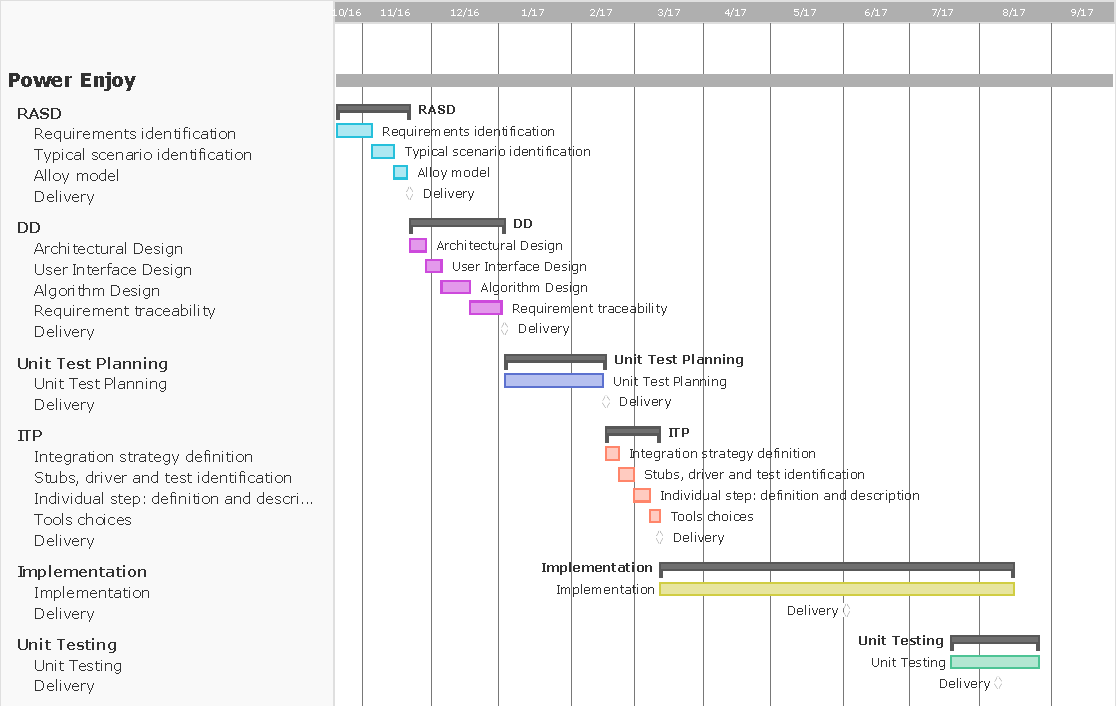
\includegraphics[width=\linewidth-1cm, keepaspectratio]{../images/Gantt.pdf}
\captionof{figure}{Gantt}
\end{minipage}

\chapter{Resources and Tasks Allocation}
The following diagram shows the allocation of resources and tasks between the three components of the development team.
The work is scheduled more or less fairly to the three components.
The reason of doing so is that especially the first phases of the project, during which is necessary to interact and to take decisions together, is difficult to assign sub tasks.
Concerning the implementation and the testing part, the work is done in parallel by the members of the team, even though every person has his/her own sub-tasks.

\begin{minipage}{\textwidth}
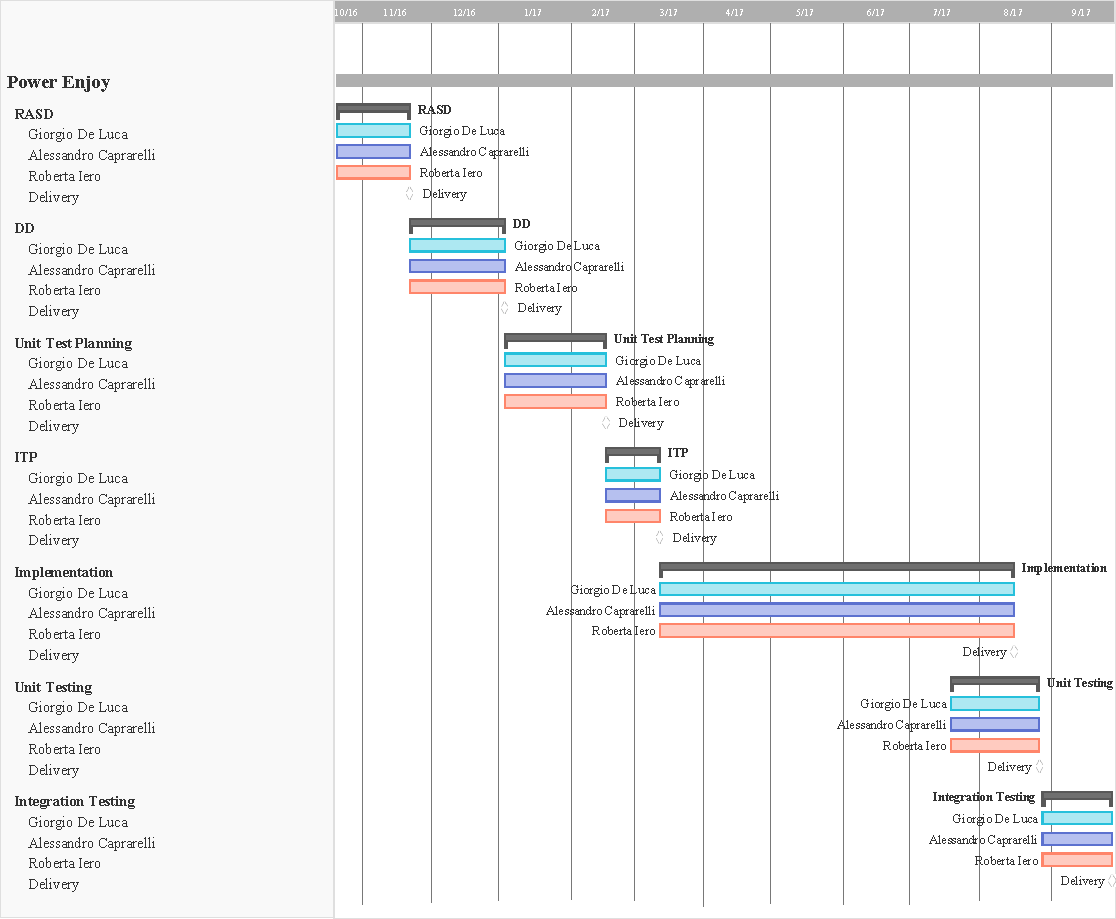
\includegraphics[width=\linewidth, keepaspectratio]{../images/resource.pdf}
\captionof{figure}{Resources allocation}
\end{minipage}

\chapter{Project risks}
In order to classify the possible risks occurring during the development process, the following probabilities related to the occur of the events are defined:
\begin{itemize}
\item Low
\item Moderate
\item High
\end{itemize}

The impacts of unexpected events are classified on the basis of the following scale:
\begin{itemize}
\item Negligible
\item Marginal
\item Serious
\item Critical
\item Catastrophic
\end{itemize}

\clearpage
\begin{table}[!h]
\centering
\caption{Project risks}
\label{project-risks}
\begin{tabularx}{\linewidth}{XXc}
\hline
\textbf{Risk}                & \textbf{Probability} & \textbf{Impact} \\ \hline
Requirements volatility      & Moderate             & Serious \\
Team cohesion                & Low                  & Critical \\
Unusability of external components & Moderate       & Critical \\
Security issues              & Low                  & Critical \\
Downtime                     & Low                  & Serious \\
Delays on project deadlines  & Moderate             & Serious \\
Lack of attractiveness of  the application & Moderate & Catastrophic \\
Integration Test Failure     & Low                  & Critical \\
Bankruptcy                   & Low                  & Catastrophic \\
Competitors                  & Moderate             & Critical \\
Use of other transports      & Moderate             & Critical \\
Changes of administrative rules and policies & Low  & Critical \\
Increase of taxes and costs of maintenance & Moderate & Marginal \\
\end{tabularx}
\end{table}

Considering the analysis done in the previous table, we illustrate for each kind of expected risk a possible strategy to adopt in order to react, whenever it’s possible.
\begin{longtable}{l|l}
\textbf{Risk}                & \textbf{Strategy}  \\ \hline
\begin{minipage}[t]{0.5\textwidth}
Requirements volatility
\end{minipage} &
\begin{minipage}[t]{0.45\textwidth}
Integrate the missing information and persuade the stakeholders to change deadlines of releases
\end{minipage} \\ \hline
\begin{minipage}[t]{0.5\textwidth}
Team cohesion
\end{minipage} &
\begin{minipage}[t]{0.45\textwidth}
A possible strategy is to clearly assign the task to each member of the team and try to encourage the communication, to maintain a relaxed environment.
\end{minipage} \\ \hline
\begin{minipage}[t]{0.5\textwidth}
Unusability of external components
\end{minipage} &
\begin{minipage}[t]{0.45\textwidth}
Solve connection problems or, in case of external services, notify as soon as possible the problem to whom it may concern
\end{minipage} \\ \hline
\begin{minipage}[t]{0.5\textwidth}
Security issues
\end{minipage} &
\begin{minipage}[t]{0.45\textwidth}
Generate a lot of focused test to analyze the behaviour of the system in different scenarios that represents bad possible behaviours of the clients
\end{minipage} \\ \hline
\begin{minipage}[t]{0.5\textwidth}
Downtime
\end{minipage} &
\begin{minipage}[t]{0.45\textwidth}
Understand the problem the causes the downtime, fix it and make the system available again
\end{minipage} \\ \hline
\begin{minipage}[t]{0.5\textwidth}
Delays on deadlines of the project
\end{minipage} &
\begin{minipage}[t]{0.45\textwidth}
Explain the causes of the delays to the stakeholders, support them in their decisions and try to not going beyond in the  future deadlines
\end{minipage} \\ \hline
\begin{minipage}[t]{0.5\textwidth}
Lack of attractiveness of the application
\end{minipage} &
\begin{minipage}[t]{0.45\textwidth}
Do a good analysis of the products of the competitors in order to identify their weaknesses and to add more features to capture the clients’ attention
\end{minipage} \\ \hline
\begin{minipage}[t]{0.5\textwidth}
Integration Test Failure
\end{minipage} &
\begin{minipage}[t]{0.45\textwidth}
Execute several tests on each single component of the system
\end{minipage} \\ \hline
\begin{minipage}[t]{0.5\textwidth}
Bankruptcy
\end{minipage} &
\begin{minipage}[t]{0.45\textwidth}
A possible strategy to prevent it is to do a correct cost estimation and a good allocation of the tasks and the resources
\end{minipage} \\ \hline
\begin{minipage}[t]{0.5\textwidth}
Competitors
\end{minipage} &
\begin{minipage}[t]{0.45\textwidth}
Add more features to the project to let it become more attractive and at the same time do a good advertising campaign
\end{minipage} \\ \hline
\begin{minipage}[t]{0.5\textwidth}
Use of other kind of means of transport
\end{minipage} &
\begin{minipage}[t]{0.45\textwidth}
Impossible to prevent. Possible solutions: acquire the new incoming business model; sell the society in time or convert it for another business model
\end{minipage} \\ \hline
\begin{minipage}[t]{0.5\textwidth}
Changes of administrative rules and policies
\end{minipage} &
\begin{minipage}[t]{0.45\textwidth}
Lobby activities
\end{minipage} \\ \hline
\begin{minipage}[t]{0.5\textwidth}
Increase of taxes and costs of maintenance
\end{minipage} &
\begin{minipage}[t]{0.45\textwidth}
Take into account during the cost estimation the possibility to save a part of the budget in order to face this problem
\end{minipage} \\ \hline
\end{longtable}




\chapter{Used tools and working hours}

\section{Used tools}

The tools used to create this document are the following:
\begin{itemize}
\item MikTex 2.9: to format the document using LaTex.
\item teamgantt.com: to create Gantt and resources allocation diagrams.
\end{itemize}

\section{Working hours}

\begin{table}[!h]
\begin{tabular}{c|c|c|c}
\centering
      & Alessandro & Roberta & Giorgio \\ \hline
14/1  &  2   &  2   &  2    \\ \hline
15/1  &  1   & 1    & 1     \\ \hline
16/1  &      &     &    \\ \hline
17/1  &  3   & 3     & 3  \\ \hline
18/1 &  1   & 1    &  1    \\ \hline
19/1 &   3   &  3    &  3  \\ \hline
20/1 &  3   & 3    & 3  \\ \hline
21/1 &  2   & 2    & 2   \\ \hline
Total & 15   & 15   & 15
\end{tabular}
\end{table}


\end{document}
